\documentclass[]{article}
\usepackage[utf8]{inputenc}
\usepackage{authblk}
\usepackage{amsmath}
\usepackage{listings}
\usepackage{float}
\usepackage{comment}
\usepackage{csquotes}
\usepackage{pgfplots}
\usepackage{hyperref}
\usepackage[%
  backend=bibtex, 
  maxbibnames=99,
  style=numeric,
  sorting=ynt,
]{biblatex}
\addbibresource{Knuth_Vol1.bib}
\addbibresource{Knuth_Vol3.bib}
\addbibresource{Cormen_Alg.bib}
\addbibresource{Die_analytische_Zahlentheorie.bib}
\addbibresource{Sareen_ComparSort.bib}
\addbibresource{Kumar_EmpiricalStudy.bib}
\addbibresource{Chhajed_CompOfFourType.bib}
\addbibresource{Aliyu_CompOnIntAndArrays.bib}
\addbibresource{Alnihoud_EnhancementMajSort.bib}
\addbibresource{Beniwal_CompOfVariousSort.bib}
\addbibresource{Ocampo_EmpiricalComp.bib}



\title{An Analytical and Experimental Comparison of Sorting Algorithms}
\author{Adrian-Ioan Tuns}
\affil{Departament of computer science

Faculty of Mathematics and Informatics

West University of Timișoara

\iffalse
Address: Bulevardul Vasile Pârvan 4, Timișoara 300223
\fi

Email: adrian.tuns99@e-uvt.ro}



\begin{document}

	\maketitle
	\begin{abstract}
Sorting is one of the fundamental issues in computer science. The purpose of this paper is to compare, both analytically and experimentally, three of the most known and used sorting algorithms, which are the following: Insertion Sort, Quick Sort and Heap Sort, thus strengthening what is already known about these algorithms regarding their complexity and behavior.

Therefore, we are going to look at the time complexity for each one of the algorithms stated above, and, furthermore, we are going to discuss the algorithms behavior for different types of data sets.
	
	\end{abstract}
	\pagebreak
	
\tableofcontents
\pagebreak

	\section{Introduction}	
Data sorting refers to any process that involves arranging the data into some meaningful order to make it easier to understand, analyze or visualize.  Sorting is particularly useful for two reasons: it helps make a set of data more readable from the human-friendly perspective and it makes it easy to search or retrieve an item from a set of data.
	
An algorithm can be defined as a series of finite steps that need to be fulfilled in a given order, such that we can accomplish the result we are seeking. Since three different sorting algorithms will be discussed, it's needless to say that the results will be different considering their time complexity, for different inputs. For more explicit and specific information about algorithms, we can look at a book where these sorting algorithms are explained thoroughly by Donald Ervin Knuth, in \textit{The Art of Computer Programming, Volume 1: Fundamental Algorithms, 3rd Edition}. For any further information, see \cite{Knuth:1997:Vol1}.

As stated before, we are going to compare three of the most common sorting algorithms, which are Insertion Sort, Quick Sort and Heap Sort. To compare these algorithms, we will run them on three types of number sequences: ascending sorted lists, decreasing sorted lists and randomly generated lists. Thus, we will be able to observe the way in which every algorithm behaves for different types of inputs, comparing them to the standards and strengthening what is already established about them.

The work described in this paper is my own work, unaided except as may be specified below and it doesn't contain material that has already been used to any substantial extent for a comparable purpose.

Regarding the paper, we will provide information on five more topics. Thus, we will give a formal description of the problem and the solution in section 2, to begin with, which means we will describe the way in which each algorithm works and it's general complexity. Having an understanding about the concept of each sorting method, we will comprehend their implementation in section 3 and see how each one of them works on the types of inputs stated above in section 4. In the end, we will go through the related work on section 5 and conclusion and future work in section 6, also giving a short summary about what has been mentioned throughout the paragraphs which will follow.
	
	\pagebreak
	
	\section{Formal Description of Problem and Solution}
To be able to talk about the complexity of an algorithm, we must first define what the $\mathcal{O}(f)$('Big $\mathcal{O}$') notations stands for. This notation has been introduced for the first time in 1894 by the German mathematician Paul Gustav Heinrich Bachmann, in his book called \textit{Die Analytische Zahlentheorie, 2nd Version}, see \cite{Bachmann:1894:Analytische}. The so called 'Big $\mathcal{O}$' notation refers to functions and their growth rate, with emphasis on how their running time or space requirements grow as the input size grows.

To make things more clear about each algorithm's efficiency regarding the number of inputs given, we will experiment on each algorithm with sequences of integer numbers in range [100-1.000.000], then we will compare the time needed for each algorithm to sort these lists, respectively.

	\subsection{Insertion Sort}
Insertion Sort is a simple sorting algorithm, which sorts numbers the same way a hand of cards would be sorted. The algorithm iterates the numbers as they follow, one at a time, and for each element in the list, the algorithm finds its correct place in the list, moves all the elements to the right and places the element in its correct place. This means that, after $n$ iterations over the initial list, the first n numbers will be sorted. 

The worst case scenario for Insertion Sort is when the elements are in descending order, because there will be one comparison for two elements, two comparisons for three elements and so on, which leads to the general case of $n$ elements, for which there will be $n-1$ comparisons. Thus, adding all these comparisons together, a general formula of $\textstyle\frac{n^2-n}{2}$ comparisons will be obtained, and, therefore, the complexity of this algorithm will be $\mathcal{O}(n^2)$, making it unsuitable for large data sets. For more information regarding Insertion Sort, see \cite{Knuth:1998:Vol3} and \cite{Cormen:2009:IAT}. 

\noindent
Insertion Sort works as follows:
\begin{center}
8, 3, 5, 1, 4

3, 8, 5, 1, 4

3, 5, 8, 1, 4

1, 3, 5, 8, 4

1, 3, 4, 5, 8
\end{center}
Thus, the list was sorted through the Insertion Sort algorithm.
	
\pagebreak

	\subsection{Quick Sort}
Quick Sort is considered to be one of the best and fastest common sorting algorithms, often being the best practical choice for sorting because it is remarkably efficient on the average. Quick Sort is an algorithm invented in 1959 by Tony Hoare, and is a Divide and Conquer based algorithm, which refers to an paradigm that solves a problem by recursively breaking down a problem into two or more sub-problems of the same or related type, until these become simple enough to be solved directly and then the sub-problems are combined to give a solution to the original problem. 

Quick Sort makes use of a certain chosen element called pivot. This pivot can be chosen randomly, from the first or the last element to the element in the middle, to any other element in the given list. Then, for the given pivot, Quick Sort will move all the elements that are smaller than the pivot to its left, and all the elements that are larger than the pivot to its right, in order to guarantee that pivot is in the correct position.
After the partitioning phase chosen the pivot, the original array will be divided into left and right arrays divided by the pivot. They will be divided even further, executing the partitioning process recursively. Dividing will be executed until one element is left in each sub-arrays, since one element is bound to locate in correct position. For the average case, Quick Sort will have the complexity of $\mathcal{O}(n\log{}n)$.

The worst case scenario for Quick Sort occurs when in each sub-arrays the smallest or greatest number is chosen as pivot, cases like that being when the array is already sorted in ascending order or in descending order. If in every partition the pivot is chosen as such, then each recursive call processes a list of size one less than the previous list, making $n-1$ passes, each sub-array having $n-i$ comparisons executed, where $i$ is the pass number. The equation will get to the general formula of $\textstyle\frac{n^2-n}{2}$, that denotes the complexity $\mathcal{O}(n^2)$. For more information about Quick Sort, see \cite{Knuth:1998:Vol3} and \cite{Cormen:2009:IAT}.

\noindent
Quick Sort algorithm works as follows:
\begin{center}
3, 2, 5, 4, 1

initial list, 5 is pivot

3, 2, 1, 4, 5

5 is in its final position, 2 is now pivot

1, 2, 4, 3, 5

2 is in its final position; on the left, there is just one element, so it is in its right position, 4 is pivot

1, 2, 4, 3, 5

3 is not in the correct place with respect to the pivot, and because there are only two remaining elements, they are swapped

1, 2, 3, 4, 5
\end{center}

\noindent
Thus, the list was sorted through the Quick Sort algorithm.
\pagebreak

	\subsection{Heap Sort}
Heap sort is a common and efficient comparison based sorting algorithm that uses the Binary Heap data structure. To define a binary heap, we much first define a binary tree, a full tree and a complete tree. A binary tree is a tree in which every parent has at most two children. A full binary tree is a binary tree in which every parent has either two or no children. A complete binary tree is a binary tree in which every level must be completely filled, and all nodes are as far left as possible. Having explained these concepts, we can now explain the concept of a binary heap. A binary heap is a complete binary tree in which every parent is either greater or smaller than its two children. If all the nodes are bigger than their children, then we call it a max-heap, and if it's the other way around, we call it a min-heap.

Heap Sort will take either the smallest or the largest element as the root, then it will swap the root with the last element and reduce the size of the list by one, such that either the largest or the smallest element will be the root, this process being repeated until all the elements have been sorted.

Heap Sort has a time complexity of $\mathcal{O}(n\log{}n)$ for all the cases(best case, average case and worst case). The height of a complete binary tree with $n$ elements is $\log n$. When applying the Heap Sort, in the worst case scenario we will need to move an element from the root to the leaf node making a multiple of $\log n$ comparisons and swaps. When building the Heap, this is done for $n/2$ elements, the complexity being $\textstyle\frac{n}{2*\log n} \simeq \log n$. During the sorting step of Heap Sort, in the worst case the applying of the sorting part will take again $\log n$. Since the building of the heap and the sorting part are executed one after another, the complexity of Heap Sort will remain $\mathcal{O}(n\log{}n)$. For further information about Heap Sort, see \cite{Knuth:1998:Vol3} and \cite{Cormen:2009:IAT}.

\noindent
Heap Sort algorithm works as follows:
\begin{center}
4, 10, 3, 5, 1

10, 4, 3, 5, 1

1, 4, 3, 5, -- 10

5, 4, 3, 1, --10

1, 4, 3, -- 5, 10

4, 1, 3 -- 5, 10

4, 3, 1, -- 5, 10

1, 3, 4, 5, 10
\end{center}

\noindent
Thus, the list was sorted through the Heap Sort algorithm.

	\pagebreak
	
	\section{Model and Implementation of Problem}
\lstset{language=C++}	
	
Regarding the implementation of these algorithms, the tests have been made using C++ language. The tests have been run on 100, 2.500, 10.000, 50.000, 100.000, 250.000, 500.000 and 1.000.000 numbers, either sorted in ascending order, in descending order or randomly generated.

The method used for measuring the time the sorting algorithms took for sorting the lists is from \lstinline!<chrono>! library from C++, which has the function
\lstinline!std::chrono::high_resolution_clock! that returns the current time with the highest precision from the \lstinline!<chrono>! methods, according to the standard.

\noindent As empirical comparison is always machine dependent, the environment where the experiments were conducted was the following: 

	Operating System: Windows 10 Home
	
	RAM: 16 GB
	
	SSD: 256 GB 
	
	Processor: i7-7700HQ CPU quad-core 2.80
	
	Compiler: CodeBlocks
	
	Language: C++

	\pagebreak
		
	\section{Test Case}
Experimentally, after running the tests on the given number of inputs, and observing how each algorithm behaves on certain types of lists stated before, we will be able to discuss the time taken by every algorithm to sort the given lists and confirm its behavior with respect to the 'Big $\mathcal{O}$' notation.

	\subsection{Ascending Sorted Lists}	
For sorted lists, Insertion Sort is the fastest, out of all the three algorithms, having a complexity of $\mathcal{O}(n)$, followed by Heap Sort, that performs in the expected $\mathcal{O}(n\log{}n)$ and then by Quick Sort, which performs the slowest, this specific case being a worst case scenario that gets to $\mathcal{O}(n^2)$ time complexity.

\bigskip
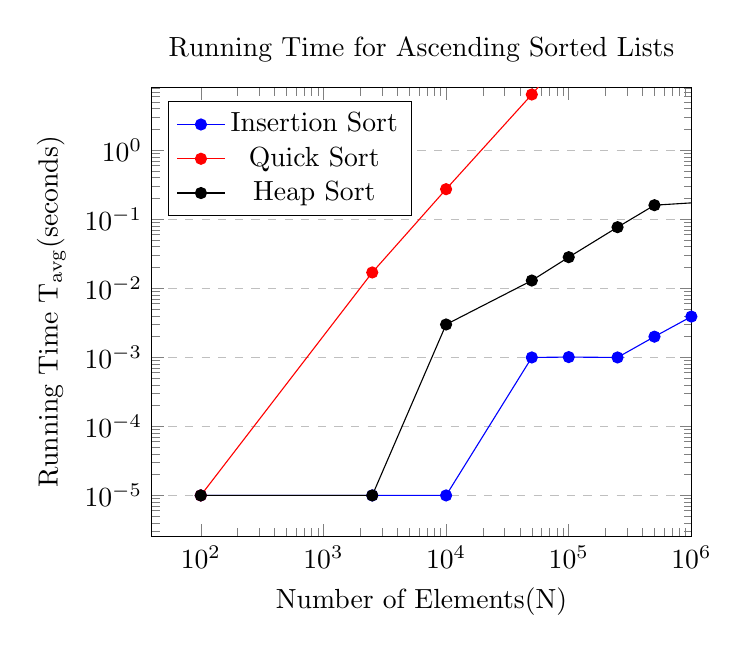
\begin{tikzpicture}
\centering
\begin{axis}[
   	title={Running Time for Ascending Sorted Lists},
    xlabel={Number of Elements(N)},
    ylabel={Running Time T\textsubscript{avg}(seconds)},
	xmode = log, ymode = log,    
    xmin=0, xmax=1000000,
    ymin=0, ymax=8,
    xtick={0,100,1000,10000,100000,1000000},
    ytick={},
    legend pos=north west,
    ymajorgrids=true,
    grid style=dashed,
]
 
\addplot[
    color=blue,
    mark=*,
    ]
    coordinates {
    (0,0)(100,0.00001)(2500,0.00001)(10000,0.00001)(50000,0.000997)(100000,0.001009)(250000,0.000997)(500000,0.001994)(1000000,0.0038986)
    };
 	\addlegendentry{Insertion Sort}
\addplot[
    color=red,
    mark=*,
    ]
    coordinates {
    (0,0)(100,0.00001)(2500,0.016966)(10000,0.272871)(50000,6.415868)(100000,26.449864)(250000,161.195339)(500000,608.42269)
    };
    \addlegendentry{Quick Sort}
 
\addplot[
    color=black,
    mark=*,
    ]
    coordinates {
    (0,0)(100,0.00001)(2500,0.00001)(10000,0.002993)(50000,0.012967)(100000,0.028249)(250000,0.076794)(500000,0.159903)(1000000000,0.374022)
    };
    \addlegendentry{Heap Sort}
    
\end{axis}
\end{tikzpicture}
\medskip

\iffalse
	INSERTION SORT
\fi

\begin{table}[H]
	\centering
\begin{tabular}{|l|l|l|l|l|}
\hline
\multicolumn{5}{|c|}{Insertion Sort} \\ \hline
N & T\textsubscript{avg}(seconds) & T\textsubscript{1}(s) & T\textsubscript{2}(s) & T\textsubscript{3}(s) \\ \hline
100 & 0.00001 & 0.00001 & 0.00001 & 0.00001 \\ \hline
2.500 & 0.00001 & 0.00001 & 0.00001 & 0.00001 \\ \hline
10.000 & 0.00001 & 0.00001 & 0.00001 & 0.00001 \\ \hline
50.000 & 0.000997 & 0.000998 & 0.000997 & 0.000998 \\ \hline
100.000 & 0.001009 & 0.001033 & 0.000998 & 0.000996 \\ \hline
250.000 & 0.000997 & 0.000998 & 0.000997 & 0.000998 \\ \hline
500.000 & 0.001994 & 0.001994 & 0.001995 & 0.001995 \\ \hline
1.000.000 & 0.003986 & 0.003987 & 0.003983 & 0.003989 \\ \hline
\end{tabular}
\end{table}

\iffalse
	QUICK SORT
\fi

\begin{table}[H]
	\centering
\begin{tabular}{|l|l|l|l|l|}
\hline
\multicolumn{5}{|c|}{Quick Sort} \\ \hline
N & Tavg & T1(s) & T2(s) & T3(s) \\ \hline
100 & 0.00001 & 0.00001 & 0.00001 & 0.00001 \\ \hline
2.500 & 0.016966 & 0.016955 & 0.016989 & 0.016954 \\ \hline
10.000 & 0.272871 & 0.273514 & 0.266316 & 0.278784 \\ \hline
50.000 & 6.415868 & 6.411452 & 6.372487 & 6.46059 \\ \hline
100.000 & 26.449864 & 27.37108 & 226.395189 & 25.583323 \\ \hline
250.000 & 161.195339 & 161.195339 & 161.195339 & 161.195338 \\ \hline
500.000 & 608.42269 & 608.278417 & 62.376517 & 608.613137 \\ \hline
1.000.000 & \multicolumn{4}{c|}{Takes too much time} \\ \hline
\end{tabular}
\end{table}

\iffalse
	HEAP SORT
\fi

\begin{table}[H]
	\centering
\begin{tabular}{|l|l|l|l|l|}
\hline
\multicolumn{5}{|c|}{Heap Sort} \\ \hline
N & T\textsubscript{avg}(seconds) & T\textsubscript{1}(s) & T\textsubscript{2}(s) & T\textsubscript{3}(s) \\ \hline
100 & 0.00001 & 0.00001 & 0.00001 & 0.00001 \\ \hline
2.500 & 0.00001 & 0.00001 & 0.00001 & 0.00001 \\ \hline
10.000 & 0.002993 & 0.002993 & 0.002992 & 0.002019 \\ \hline
50.000 & 0.012967 & 0.012964 & 0.012969 & 0.012969 \\ \hline
100.000 & 0.028249 & 0.028923 & 0.027912 & 0.027912 \\ \hline
250.000 & 0.076794 & 0.076794 & 0.073802 & 0.076794 \\ \hline
500.000 & 0.159903 & 0.158603 & 0.160553 & 0.160553 \\ \hline
1.000.000 & 0.374022 & 0.369984 & 0.376042 & 0.376042 \\ \hline
\end{tabular}
\end{table}

	\pagebreak
	
	\subsection{Descending Sorted Lists}
For descending sorted lists, Heap Sort is the fastest, with its usual complexity of $\mathcal{O}(n\log{}n)$, Insertion Sort and Quick Sort both taking too much time, both of them having an $\mathcal{O}(n^2)$ complexity. However, Quick Sort performs worse than Insertion Sort, being the slowest of the three presented algorithms for this specific type of input lists.

\bigskip
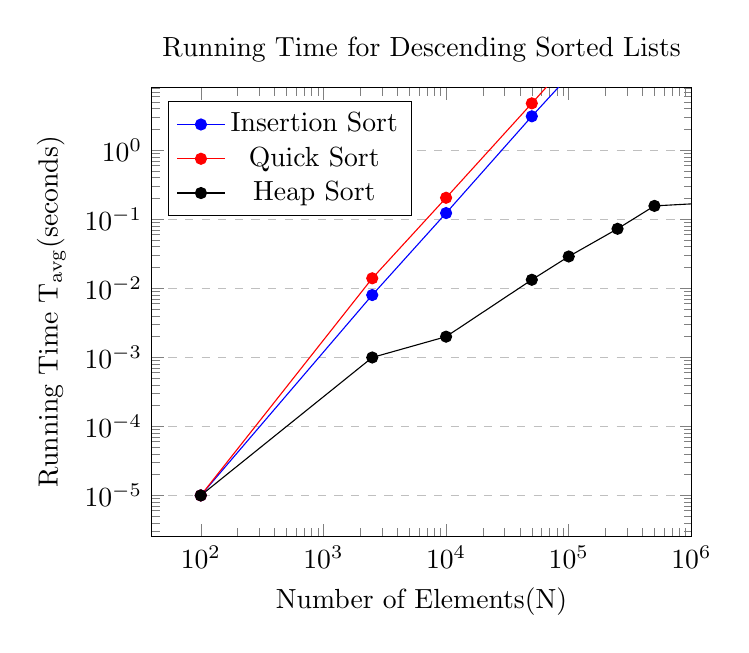
\begin{tikzpicture}
\centering
\begin{axis}[
   	title={Running Time for Descending Sorted Lists},
    xlabel={Number of Elements(N)},
    ylabel={Running Time T\textsubscript{avg}(seconds)},
	xmode = log, ymode = log,    
    xmin=0, xmax=1000000,
    ymin=0, ymax=8,
    xtick={0,100,1000,10000,100000,1000000},
    ytick={},
    legend pos=north west,
    ymajorgrids=true,
    grid style=dashed,
]
 
\addplot[
    color=blue,
    mark=*,
    ]
    coordinates {
    (0,0)(100,0.00001)(2500,0.007992)(10000,0.123008)(50000,3.099069)(100000,11.860596)(250000,73.638882)(500000,289.345398)(1000000,1134.02489)
    };
 	\addlegendentry{Insertion Sort}
\addplot[
    color=red,
    mark=*,
    ]
    coordinates {
    (0,0)(100,0.00001)(2500,0.013963)(10000,0.20481)(50000,4.775166)(100000,18.727545)(250000,115.963671)(500000,451.334676)
    };
    \addlegendentry{Quick Sort}
 
\addplot[
    color=black,
    mark=*,
    ]
    coordinates {
    (0,0)(100,0.00001)(2500,0.000996)(10000,0.001995)(50000,0.013297)(100000,0.028917)(250000,0.072809)(500000,0.156257)(1000000000,0.325122)
    };
    \addlegendentry{Heap Sort}
    
\end{axis}
\end{tikzpicture}
\medskip

\iffalse
	INSERTION SORT
\fi
	
\begin{table}[H]
	\centering
\begin{tabular}{|l|l|l|l|l|}
\hline
\multicolumn{5}{|c|}{Insertion Sort} \\ \hline
N & T\textsubscript{avg}(seconds) & T\textsubscript{1}(s) & T\textsubscript{2}(s) & T\textsubscript{3}(s) \\ \hline
100 & 0.00001 & 0.00001 & 0.00001 & 0.00001 \\ \hline
2.500 & 0.007992 & 0.007978 & 0.007998 & 0.008001 \\ \hline
10.000 & 0.123008 & 0.126633 & 0.119695 & 0.122698 \\ \hline
50.000 & 3.099069 & 3.185468 & 3.034932 & 3.076807 \\ \hline
100.000 & 11.860596 & 11.877213 & 1.859287 & 11.845288 \\ \hline
250.000 & 73.638882 & 74.345161 & 72.882459 & 73.68026 \\ \hline
500.000 & 289.345398 & 289.727258 & 289.233998 & 289.456798 \\ \hline
1.000.000 & 1 134.02489 & 1 134.0649 & 1 134.01189 & 1 134.02659 \\ \hline
\end{tabular}
\end{table}

\iffalse
	QUICK SORT
\fi

\begin{table}[H]
	\centering
\begin{tabular}{|l|l|l|l|l|}
\hline
\multicolumn{5}{|c|}{Quick Sort} \\ \hline
N & Tavg & T1(s) & T2(s) & T3(s) \\ \hline
100 & 0.00001 & 0.00001 & 0.00001 & 0.00001 \\ \hline
2.500 & 0.013963 & 0.013965 & 0.013962 & 0.013963 \\ \hline
10.000 & 0.20481 & 0.206447 & 0.200514 & 0.207469 \\ \hline
50.000 & 4.775166 & 4.889424 & 4.70195 & 4.734125 \\ \hline
100.000 & 18.727545 & 18.612291 & 18.830274 & 18.74007 \\ \hline
250.000 & 115.963671 & 115.54805 & 115.849477 & 116.493486 \\ \hline
500.000 & 451.334676 & 451.319343 & 451.428373 & 451.256313 \\ \hline
1.000.000 & \multicolumn{4}{c|}{Takes too much time} \\ \hline
\end{tabular}
\end{table}

\iffalse
	HEAP SORT
\fi


\begin{table}[H]
	\centering
\begin{tabular}{|l|l|l|l|l|}
\hline
\multicolumn{5}{|c|}{Heap Sort} \\ \hline
N & T\textsubscript{avg}(seconds) & T\textsubscript{1}(s) & T\textsubscript{2}(s) & T\textsubscript{3}(s) \\ \hline
100 & 0.00001 & 0.00001 & 0.00001 & 0.00001 \\ \hline
2.500 & 0.000996 & 0.000996 & 0.000997 & 0.000996 \\ \hline
10.000 & 0.001995 & 0.00199 & 0.002003 & 0.001994 \\ \hline
50.000 & 0.013297 & 0.012969 & 0.012959 & 0.013964 \\ \hline
100.000 & 0.028917 & 0.028961 & 0.02887 & 0.028922 \\ \hline
250.000 & 0.072809 & 0.07383 & 0.071808 & 0.072791 \\ \hline
500.000 & 0.156257 & 0.155585 & 0.156611 & 0.156575 \\ \hline
1.000.000 & 0.325122 & 0.313163 & 0.327099 & 0.33104 \\ \hline
\end{tabular}
\end{table}

	\pagebreak
	
	\subsection{Randomly Generated Lists}
In the case of randomly generated lists, Quick Sort has the best performance out of all the previously stated algorithms, followed by Heap Sort and Insertion Sort, Quick Sort having an average time of 0.19371 seconds for 1.000.000 elements, compared to 0.507236 seconds of Heap Sort and the substantial time of 614.71654 seconds for Insertion Sort, the average complexity of Insertion Sort being $\mathcal{O}(n^2)$, compared to $\mathcal{O}(n\log{}n)$ of Quick Sort and Heap Sort.

\bigskip
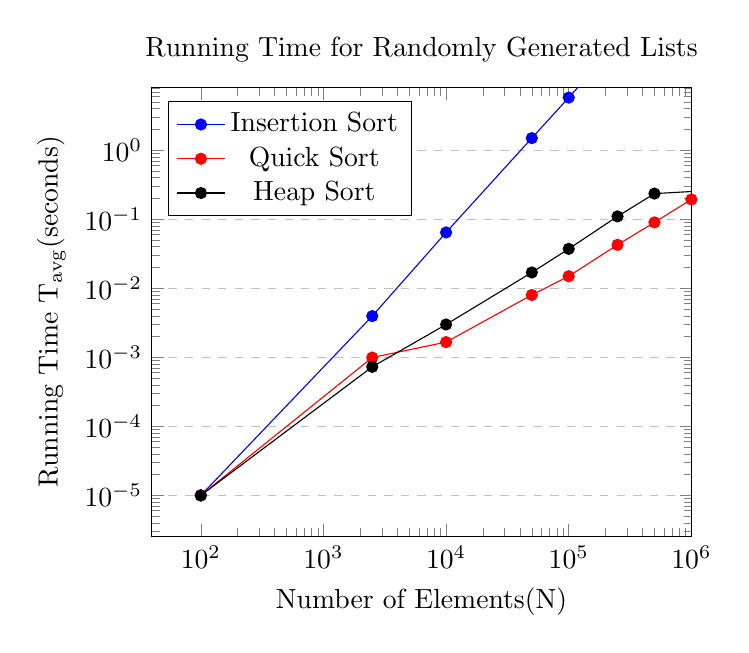
\begin{tikzpicture}
\centering
\begin{axis}[
   	title={Running Time for Randomly Generated Lists},
    xlabel={Number of Elements(N)},
    ylabel={Running Time T\textsubscript{avg}(seconds)},
	xmode = log, ymode = log,    
    xmin=0, xmax=1000000,
    ymin=0, ymax=8,
    xtick={0,100,1000,10000,100000,1000000},
    ytick={},
    legend pos=north west,
    ymajorgrids=true,
    grid style=dashed,
]
 
\addplot[
    color=blue,
    mark=*,
    ]
    coordinates {
    (0,0)(100,0.00001)(2500,0.003961)(10000,0.064499)(50000,1.497652)(100000,5.788853)(250000,35.427842)(500000,141.05064)(1000000,614.71654)
    };
 	\addlegendentry{Insertion Sort}
\addplot[
    color=red,
    mark=*,
    ]
    coordinates {
    (0,0)(100,0.00001)(2500,0.000994)(10000,0.001663)(50000,0.008012)(100000,0.014959)(250000,0.042656)(500000,0.090138)(1000000,0.19371)
    };
    \addlegendentry{Quick Sort}
 
\addplot[
    color=black,
    mark=*,
    ]
    coordinates {
    (0,0)(100,0.00001)(2500,0.000729)(10000,0.002992)(50000,0.016963)(100000,0.037242)(250000,0.110111)(500000,0.235308)(1000000000,0.507236)
    };
    \addlegendentry{Heap Sort}
    
\end{axis}
\end{tikzpicture}
\medskip

\iffalse
	INSERTION SORT
\fi
	
\begin{table}[H]
	\centering
\begin{tabular}{|l|l|l|l|l|}
\hline
\multicolumn{5}{|c|}{Insertion Sort} \\ \hline
N & T\textsubscript{avg}(seconds) & T\textsubscript{1}(s) & T\textsubscript{2}(s) & T\textsubscript{3}(s) \\ \hline
100 & 0.00001 & 0.00001 & 0.00001 & 0.00001 \\ \hline
2.500 & 0.003961 & 0.003988 & 0.0049906 & 0.002991 \\ \hline
10.000 & 0.064499 & 0.066822 & 0.060846 & 0.065831 \\ \hline
50.000 & 1.497652 & 1.495993 & 1.486008 & 1.510956 \\ \hline
100.000 & 5.788853 & 5.868278 & 5.834413 & 5.663869 \\ \hline
250.000 & 35.427842 & 35.504962 & 35.479082 & 35.299484 \\ \hline
500.000 & 141.05064 & 141.685831 & 140.786246 & 140.679845 \\ \hline
1.000.000 & 614.71654 & 614.7496 & 614.6998 & 614.71228 \\ \hline
\end{tabular}
\end{table}

\iffalse
	QUICK SORT
\fi

\begin{table}[H]
	\centering
\begin{tabular}{|l|l|l|l|l|}
\hline
\multicolumn{5}{|c|}{Quick Sort} \\ \hline
N & T\textsubscript{avg}(seconds) & T\textsubscript{1}(s) & T\textsubscript{2}(s) & T\textsubscript{3}(s) \\ \hline
100 & 0.00001 & 0.00001 & 0.00001 & 0.00001 \\ \hline
2.500 & 0.000994 & 0.000985 & 0.001004 & 0.000994 \\ \hline
10.000 & 0.001663 & 0.001993 & 0.001004 & 0.001994 \\ \hline
50.000 & 0.008012 & 0.00803 & 0.007974 & 0.008034 \\ \hline
100.000 & 0.014959 & 0.014936 & 0.01496 & 0.014982 \\ \hline
250.000 & 0.042656 & 0.041839 & 0.043735 & 0.042394 \\ \hline
500.000 & 0.090138 & 0.090757 & 0.091986 & 0.087673 \\ \hline
1.000.000 & 0.19371 & 0.197454 & 0.19948 & 0.187941 \\ \hline
\end{tabular}
\end{table}

\iffalse
	HEAP SORT
\fi


\begin{table}[H]
	\centering
\begin{tabular}{|l|l|l|l|l|}
\hline
\multicolumn{5}{|c|}{Heap Sort} \\ \hline
N & T\textsubscript{avg}(seconds) & T\textsubscript{1}(s) & T\textsubscript{2}(s) & T\textsubscript{3}(s) \\ \hline
100 & 0.00001 & 0.00001 & 0.00001 & 0.00001 \\ \hline
2.500 & 0.000729 & 0.0001064 & 0.001047 & 0.001035 \\ \hline
10.000 & 0.002992 & 0.002991 & 0.002992 & 0.002995 \\ \hline
50.000 & 0.016963 & 0.016955 & 0.016956 & 0.016978 \\ \hline
100.000 & 0.037242 & 0.036877 & 0.036951 & 0.0379 \\ \hline
250.000 & 0.110111 & 0.110426 & 0.110211 & 0.109698 \\ \hline
500.000 & 0.235308 & 0.230438 & 0.232378 & 0.243109 \\ \hline
1.000.000 & 0.507236 & 0.501441 & 0.494676 & 0.525593 \\ \hline
\end{tabular}
\end{table}

	\pagebreak

	\section{Related Work}
	
Jehad Alnihoud and Rami Mansi state that sorting is graded as a fundamental problem in computer science \cite{alnihoud2010enhancement}. Sonal Beniwal and Deepti Groover, concluded that the quality of a good sorting algorithm is not only represented by the speed of sorting but by other factors too, as the length, the code complexity, stability, performance consistency and the handling of specific data time \cite{beniwal2013comparison}. This conclusion was drawn after an comparison of Bubble, Heap, Insertion, Merge and Quick Sort algorithms.

Aliyu Ahmed and Dr. Zirra in \cite{aliyu2013comparative} have compared Insertion Sort and Quick Sort algorithms on both integer and character arrays concluding that performance of Insertion Sort is better than Quick Sort. Both algorithms were used for sorting a small number of items. Also, CPU time consumption while sorting integer arrays was very low compared to an input of character arrays. In \cite{chhajed2013comparison} Nidhi Chhajed and Simarjeet Singh Bhatia concluded that Insertion Sort algorithm is slower than Heap Sort and Quick Sort, after comparing Quick, Heap and Insertion Sort algorithms in terms of time complexity and various performance factors. Random numbers between 10.000 to 30.000 have been used as input data. Both Insertion Sort and Quick Sort have worst case time complexity of $\mathcal{O}(n^2)$, Heap Sort having $\mathcal{O}(nlog{}n)$ time complexity. Quick Sort performed better than the other two. As the input increases Insertion Sort performs very poorly and shows an exponential growth. 

In \cite{kumar2013empirical} G. Kumar and H. Ghugh have compared Bubble, Insertion, Quick, Merge and Heap sorting algorithms on 100.000, 300.000, 500.000, 700.000, 1.000.000, 1.500.000 input values. After comparing the data empirically the algorithms were ranked in the following order on the basis of their speed: Merge, Quick, Heap, Insertion and Bubble Sort. It was concluded that Merge, Quick and Heap Sort algorithms are faster than the remaining two when the input size is very large. 

In \cite{sareen2013comparison} Pankaj Sareen has compared Bubble, Insertion, Selection, Merge and Quick Sort algorithms on the input values of 10, 100, 1.000 and 10.000 elements. The comparison was based on average case only. The average running time of all the algorithms was noted on these inputs and presented graphically. It was concluded that the most efficient algorithm was Quick Sort. In \cite{Cormen:2009:IAT} and \cite{ocampo2008empirical} several studies suggest that all algorithms perform $\mathcal{O}(n^2)$ in their worst case scenario, Quick Sort being the only algorithm which has an average and best run-time of $\mathcal{O}(n\log{}n)$. This concludes that Quick Sort is better than Insertion, Bubble and Selection Sort in average case, for sufficiently large input. 

	\pagebreak
		
	\section{Conclusion and Future Work}
As a conclusion, we can say that we have confirmed what was known previously and strengthened the results through the experiments we have previously discussed. Thus, for specific types of inputs, such as ascending sorted lists and descending sorted lists, Quick Sort takes way too much time to compile and analyze the given list, reinforcing what was known about the worst case scenario of this algorithm, along with Insertion Sort in the case of descending sorted lists, this being the worst case scenario for Insertion Sort. Quick Sort is the fastest out of the sorting algorithms when the input given is a randomly generated list. Heap Sort performs in an expected manner, the inputs being sorted fast, without taking into consideration whether the elements are sorted or not.

Generally speaking, for a randomly sorted list, Insertion Sort is the most inefficient, whereas Heap Sort and Quick Sort return the sorted list almost immediately, even for a million numbers list.

The tests run and explained in this paper show only a small part of the whole, big result. We have only discussed about three, most common cases, on integer data types, which are ascending sorted lists, descending sorted lists and randomly generated lists, out of all the possible cases that there are, which haven't been covered, but these cases will be analyzed and discussed in future works.

	\pagebreak	
	
\printbibliography

\addcontentsline{toc}{section}{References}

\end{document}